% ************************************************
\chapter{Network Model}\label{ch:Network Model} 
% ************************************************

Referring to anisotropic characteristics in local cortical circuits of
the rat's brain, a network model implementing anisotropic tissue
geometry is developed. The introduction of a rewiring algorithm and
qualitative anisotropy measure %quantitative ??
lay the foundation for the analysis of structural aspects of this
model in Chapter~\ref{ch:structural_aspects}.

\parskip = \baselineskip %??
\setlength{\parindent}{0pt}

%\section{Introduction}\label{sec:intro_model}
\clearpage
\section{Anisotropy in Neural Connectivity}\label{sec:biol_anisotropy}

% The field of neurogeometry is trying to answer the question when
% synaptic connections . Several studies
% report \parencite{Stepanyants2005}
% Axonal and synaptic is uncorrelated \parencite{Stepanyants2005} 

% The main stem of a pyramidal cell's axon , laying the foundation for
% anisotropy in connectivity.



% Research in the field of neurogeometry yields a simple rule for
% networks to be connected 

% Thus axon morphology distinctively determines network 
% connectivity. \marginpar{axon
% morphology determines connectivity}

Neurogeometry\index{neuro geometry} addresses the problem of inferring
synaptic connectivity from the geometric shapes of axon and
dendrites. A fundamental concept in this field is that of a
\textit{potential synapse}\index{potential synapse}
\parencite{Stepanyants2002}. Defined as the potential axonal-dendritic
connection of two neurons, present whenever the axon of one neuron is
within a spatial distance $s$ of the dendrite of the other, it is a
necessary, although not sufficient, condition for the formation of a
synaptic connection (\autoref{fig:potential_synapse}). The existence
of such close appositions solely depends on dendritic and axonal
anatomy; identification of defining morphological characteristics in
both axon and dendrite would therefore allow for a model of local
network connectivity, assuming for example that a certain ratio $r$ of
potential synapses turn into active contacts independently. It is the
hope that such a model, motivated from the geometry of a neuron's
functional compartments, not only displays inherent patterns of
connectivity similar to what has been observed in biological networks,
but also proofs itself as a testing ground for how this connectivity
may affect network dynamics.

\vspace{-0.25cm}
\definecolor{lightgray}{rgb}{0.88, 0.88, 0.88}
\begin{center}
 \setlength{\fboxrule}{0pt}
 \fcolorbox{black}{lightgray}{
   \begin{minipage}[c]{0.90\textwidth}

     \vspace{0.1cm}
     \setlength{\intextsep}{0pt}%
     \setlength{\columnsep}{8pt}%
     \begin{wrapfigure}{r}{0.65\textwidth}
       \captionsetup{labelformat=empty,labelsep=none}
       \centering
       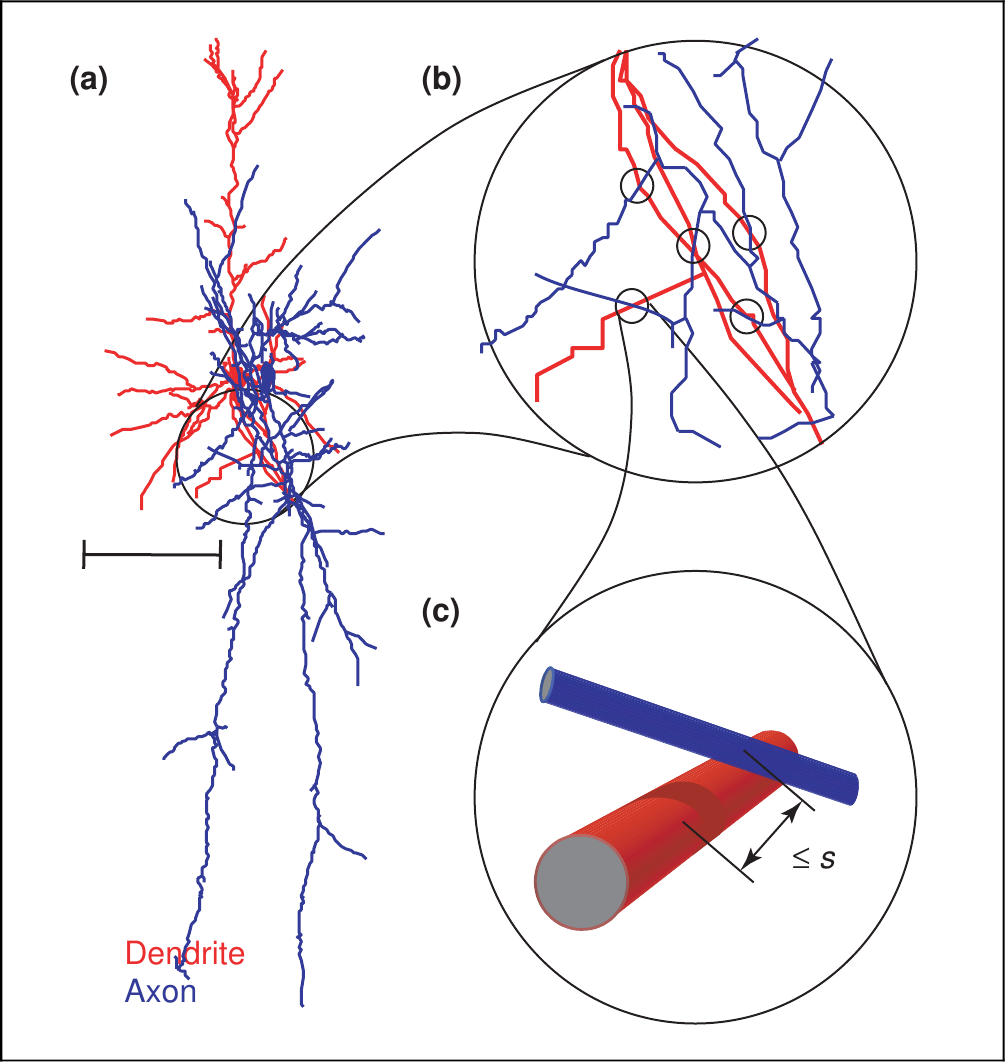
\includegraphics[width=\linewidth]{img/potential_synapse2.png}
       \vspace{-35pt}
       \caption{}
       \label{fig:potential_synapse}
     \end{wrapfigure}

     \footnotesize \textbf{Potential Synapse} 
     \smallskip

     Close ap\-positions be\-tween den\-drite and axon
     are a necessary condition for the formation of a synapse. \textbf{(a)}
     3-D reconstructions of a py\-ra\-mi\-dal cell den\-drite in red, axon of a
     regular spiking non-pyramidal cell in blue. \textbf{(b)-(c)}
     Overlapping arbors allow for several potential synapses whenever
     dendrite and axon are within a spatial distance $\leq s$. Values for
     $s$ depend on the type of synapse, typically between
     0.4-\SI{2}{\micro\meter}. Scale bar: \SI{100}{\micro\meter},
     \SI{30}{\micro\meter}, \SI{3}{\micro\meter} in (a),(b),(c)
     respectively. Image from \textcite{Stepanyants2005}. \hfill \textbf{4.1}

     \vspace{0.1cm}
   \end{minipage}}
\end{center}


% \vspace{0.5cm}
% \begin{figure}[!htbp] 
%   \centering 
%   \includegraphics[width=0.55\textwidth]{%
%     img/potential_synapse1.png}%
%   \caption{\textbf{Tracing axonal branching of a pyramidal cell}.}%?? not the right caption    
%   \label{fig:potential_synapse}
% \end{figure}

% \vspace{0.5cm}
% \begin{figure}[!htbp]
% \captionsetup{format=plain}
% \floatbox[{\capbeside\thisfloatsetup{capbesideposition={right,top},capbesidewidth=0.3\textwidth}}]{figure}[\FBwidth]
% {\includegraphics[width=0.6\textwidth]{img/potential_synapse1.png}}
% {%
%   \caption{\textbf{Potential Synapse} Close appositions between
%           dendrite and axon are a necessary condition for the formation of a
%           synapse. \textbf{(a)} 3-D reconstructions of a pyramidal cell dendrite
%           in red, axon of a regular spiking non-pyramidal cell in
%           blue. \textbf{(b)-(c)} Overlapping arbors allow
%           for several potential synapses whenever dendrite and axon are within a
%           spatial distance $\leq s$. Values for $s$ depend on the type of
%           synapse, typically between 0.4-\SI{2}{\micro\meter}. Scale bar:
%           \SI{100}{\micro\meter}, \SI{30}{\micro\meter}, \SI{3}{\micro\meter} in
%           (a),(b),(c) respectively. Image from
%           \textcite{Stepanyants2005}.}%
%   \label{fig:potential_synapse}%
% }
% \end{figure}                                
% \vspace{0.3cm}


Finding stereotypical anatomical characteristics however is difficult,
as axonal morphology is, in general, highly diverse
%------------------------------------------------
\marginpar{high variability in axonal morphology} 
%------------------------------------------------ 
\parencite{Debanne2004}. Across different species,
distinct regions in the central nervous system and different neuron
types, axons display a wide variety of shapes characterized by
morphometric parameters such as total length, branching complexity and
axonal extent \parencite{Ropireddy2011}. Typical examples of distinct
morphology include the T-shaped axons of cerebellar granule cells
branching only at a singular point \parencite{Cajal1911}, and axons of hippocampal CA3
pyramidal cells, which, in stark contrast, may feature up to 40
branches resulting in a total length of axon collaterals of up to
\SI{12}{\milli\meter} \parencite{Ishizuka1990}.

It is therefore imperative to confine this analysis to a specific
brain region and neuron type. In this study, we set the focus on
circuits of pyramidal cells in the mammalian cortex.
%?? Cortex does this
%?? Cortex is this well studied
%?? Here we go
More specifically, local circuits of thick tufted layer V
pyramidal neurons in the rat's somatsosensory cortex have been the
target of advanced
experimentation \parencite{Song2005,Perin2011,Romand2011, Ramaswamy2012}, and will
serve as a benchmark for results in neural morphology and network
connectivity in this report.

\begin{figure}[!htbp]
  \centering 
  \makebox[0.875\textwidth]{%
    \begin{overpic}[width=0.4\textwidth]{%
        img/network_model/p14rr_1.pdf}
      \put(3,92){\small\textbf{A}}
    \end{overpic}
    \hfill
    \begin{overpic}[width=0.4\textwidth]{%
        img/network_model/p14rr_1_axon_traced_soma.pdf}
      \put(3,92){\small\textbf{B}}
    \end{overpic}
    }%
  \caption{\textbf{Tracing axonal branching of a pyramidal cell} In a
    3-D model reconstructed from biocytin-labeled thick-tufted layer V
    pyramidal cells in the somatosensory cortex of postnatal (day 14)
    Wistar rats, \textcite{Romand2011} depict dendritic compartments in
    red, axonal compartments in blue.  \textbf{A)} A
    \SI{600}{\micro\meter} window centered on the soma of the pyramidal
    cell shows the main stem of the cell's axon projecting downwards in a
    straight line, collaterals branching at various angles. \textbf{B)}
    Using image manipulation software, axon morphology was manually traced
    and is emphasized in black.}    
  \label{fig:romand_axon_trace}
\end{figure}
\vspace{-0.2cm}

Axonal morphology of pyramidal cells in the cerebral cortex is well
described. From the soma the single main stem of the axon
%------------------------------------------------
\marginpar{cortical axons form straight lines, arborize profusely} 
%------------------------------------------------ 
originates and projects downwards, describing a trajectory closely
resembling a straight line \parencite{Braitenberg_Cortex}. At
arbitrary points along this path, collaterals branch off at various
angles and constitute themself linear paths until they further ramify
or terminate. Displaying a high degree of ramification, axonal trees
of cortical pyramidal cells build, in general, complex
structures \parencite{Petersen2003,Ramaswamy2012}. Cortical slice
experiments analyzing neural anatomy are typically constrained by a
slice thickness of \SI{300}{\micro\meter}. On this scale, 3-D
reconstruction from labeled thick tufted layer V pyramidal cells
reveals characteristic morphology of the axonal tree
(\autoref{fig:romand_axon_trace}). The downwards projecting, straight
axon branches at several points, forming collateral branches that
travel in linear path as well.

In a statistical view, this characteristic axonal morphology results
in high axon branch densities along the main stem, whereas distant
regions display a relatively low density
(\autoref{fig:axon_heat}). Specifically, axon collaterals do not
cluster around the soma but align with the main stem's projection. As
presence of an axonal branch constitutes a necessary condition for a
potential synapse, a higher concentration of potential and,
subsequently, realized synapses is expected in regions of high branch
density. For a coherent picture of local connectivity profiles,
however, dendritic morphology needs to be considered as well. 

 
\begin{figure}[!htbp]
  \centering 
  \makebox[0.875\textwidth]{%
    \begin{overpic}[width=0.4\textwidth]{img/network_model/p14rr_1_trace_soma.pdf}
      \put(3,92){\small\textbf{A}}
    \end{overpic}
    \hfill
    \begin{overpic}[width=0.4\textwidth]{img/network_model/axon_heat_correct_soma.png}
      \put(3,92){\small\textbf{\textcolor{white}{B}}}
    \end{overpic}
    }%
    \caption{%
      \textbf{Illustrating axonal branch density}
      In a sample of 5 reconstructions from thick-tufted layer V pyramidal
      cells \parencite{Romand2011}, tracing axonal morphology illustrates
      characteristic branch density along the axon's main
      stem. \textbf{A)} Example of extracted axonal tree. Outline manually
      traced using image manipulation software. Soma indicated by
      triangle. Original data from \textcite{Romand2011}. \textbf{B)}
      Overlaying 5 axonal trees extracted as in A), 
      % ?? show Appendix?  Sumatra label?? colorbar??
      applying a Gaussian filter and displaying high axon densities in
      warm colors, illustrates the characteristic higher branch
      densities along the axon's main stem.}
  \label{fig:axon_heat}
\end{figure}
\vspace{-0.2cm}

Dendritic anatomy of cortical pyramidal cells is inherently bipartite.
From the soma several \textit{basal dendrites}\index{basal dendrite}
emerge and extend into arbitrary directions, branching profusely until
they terminate . The single \textit{apical dendrite}\index{apical
  dendrite} emerges from the apex of the pyramidal cell and ascends in
a linear trajectory, forming occasional collateral branches until
finally terminating into the apical tuft, where the dendrite branches
several times to form a tree like structure \parencite{Feldman1984}.
%------------------------------------------------
\marginpar{basal dendrites dominate local connectivity} 
%------------------------------------------------  
On the scale of typical cortical slice thickness, however, the apical
dendrite is cut off and the basal dendrite dominates the dendritic
morphology and potential of dendritic-axonal connections
(\autoref{fig:dendrite_heat}). The radial extension of dendritic
branches results in a high concentration of dendritic branches around the
soma, much in the contrast to the findings of axonal branch densities
before.

\begin{figure}[!ht]
  \makebox[0.875\textwidth]{%
    \begin{overpic}[width=0.4\textwidth]{%
        img/network_model/p14rr_1.pdf}
      \put(3,92){\small\textbf{A}}
    \end{overpic}
    \hfill
   \begin{overpic}[width=0.4\textwidth]{img/network_model/p14rr_1_traced_soma.pdf}
      \put(3,92){\small\textbf{B}}
    \end{overpic}
    }
  \vfill
  \vspace{0.3cm}
  \makebox[0.875\textwidth]{%
    \begin{overpic}[width=0.4\textwidth]{img/network_model/p14rr_1_dendrite_trace_scale.pdf}
      \put(3,92){\small\textbf{C}}
    \end{overpic}
    \hfill
    \begin{overpic}[width=0.4\textwidth]{img/network_model/dendrite_heat_correct_soma.png}
      \put(3,92){\small\textbf{\textcolor{white}{D}}}
    \end{overpic}
    }%
  \caption{\textbf{Dendritic morphology and branch density}
    Using neuronal morphology of thick-tufted layer V
    pyramidal cells recorded by \textcite{Romand2011}, dendritic
    anatomy is traced and combined to illustrate high
    branch density around the soma. \textbf{A)} In a
    \SI{600}{\micro\meter} window centered on the soma, basal
    dendrites (red) are visible extending around the soma. The ascending
    thick apical dendrite (red) is cut off and apical tuft is not
    shown. \textbf{B)-C)} Manual tracing of dendritic outlines
    in five samples (one shown), allows for clearer identification of
    stereotypical morphology and later analysis. \textbf{D)} Combining
    5 dendritic outlines as shown in C) and subsequent Gaussian
    filtering reveals the relatively high dendritic branch density
    around the soma.
  }%?? sumatra label
  \label{fig:dendrite_heat}
\end{figure}
\vspace{-0.2cm}

Combining the above results of dendritic and axonal branch densities
in the light of neurogeometry, a clear concept of anisotropy of neural
connectivity emerges. As dendritic branches of potential post-synaptic
targets extend radially from the soma and do not display a preferred
direction, target neurons for outgoing synaptic contacts originating
from a single pyramidal cell, cluster around the downwards projecting
axon (\autoref{fig:neural_anisotropy}). %?? high branch density
                                %correlates directly with expected
                                %number of contacts!
\begin{figure}[!ht]
  \centering 
  \makebox[0.875\textwidth]{%
    \begin{overpic}[width=0.4\textwidth,frame]{img/network_model/axon_dendrite_meet.pdf}
      \put(3,92){\small\textbf{A}}
    \end{overpic}
    \hfill
    \begin{overpic}[width=0.4\textwidth,frame]{img/network_model/axon_dendrite_meet_schema_dense.pdf}
      \put(3,92){\small\textbf{B}}
    \end{overpic}
    }%

    \caption{%
      \textbf{Connected neurons of a single pyramidal cell align with
        axonal projection} Reducing the full axonal (blue,
      cf. \autoref{fig:romand_axon_trace}) and dendritic trees (red, gray,
      cf. \autoref{fig:dendrite_heat}) as shown for two neurons in A)
      to their stereotypical axonal (blue) and dendritic profiles
      (red, gray) in B), demonstrates how connected neurons (red) tend
      to cluster around the pre-synaptic axon's profile, as spatial
      closeness constitutes a necessary condition for the formation of
      contacts. Unconnected neurons (gray) are found distant from the
      axon's projection, but not necessarily distant from the soma. }
  \label{fig:neural_anisotropy}
\end{figure}
%\vspace{-0.2cm} 
% Why is anisotropy so good??
% It becomes apparent that
% connected neurons are located along the main axon in much higher
% concentration than in directions that diverge from the axon's
% projection. 
In their in-depth study, \textcite{Stepanyants2005} confirm the
overrepresentation of potential synapses along the axon for pyramidal
cells. Consistent with the notion that stereotypical morphology of
pyramidal cells is intrinsic to the local network's connectivity
profile, they also find that anisotropy of this degree is \textit{not}
present in spiny stellate neurons located in lower-layer-4.



% It is worth noting that this result of anisotropic connectivity does,
% in general, not hold for other brain regions and neurons type. While
% the ad hoc approach taken here is confirmed by an in-depth study of
% \textcite{Stepanyants2005} for cortical pyramidal cells, spiny
% stellate neurons located in lower-layer-4 do not show a clear
% preferred direction for potential synapse.


% Thick tufted pyramidal cells in the rat's somatosensory cortex 

% Owing to this diversity, it is impossible to and it
% is our intent to focus on a specific neuron type and brain region.

% Neuron morphology as well as network connectivity in the rat's
% somatosensory cortex has been thoroughly studied. Even more
% specifically, thick tufted layer V have been the target of studies. 
% \marginpar{focus on TTL5 neurons}


% Neuron morphology and connectivity in the rat's somatosensory cortex
% has been thoroughly studied. As s. 




% the respective axonal
% trees where traced using image manipulation o 

% , showing an apparent anisotropy in neural connectivity, aligning with
% the growth direction of axon's main stem (\autoref{fig:axon_heat}).


% Combing the heatmaps, we obtain clear evidence for anisotropy. In the
% next section we will combine dendritic and axonal morphological
% characteristics into an abstracted geometric model. 

% Identifying anisotropy in neural connectivity as an interesting . In
% this thesis 
% In this study is more specifically focusing in pyramidal neurons in 


% \vspace{0.5cm}
% \begin{figure}[h] 
%   \centering 
%   \makebox[0.875\textwidth]{%
%     \begin{overpic}[width=0.4\textwidth]{img/network_model/p14rr_1_trace_soma.pdf}
%       \put(3,92){\small\textbf{A}}
%     \end{overpic}
%     \hfill
%     \begin{overpic}[width=0.4\textwidth]{img/network_model/p14rr_1_trace_soma.pdf}
%       \put(3,92){\small\textbf{B}}
%     \end{overpic}
%     }%
%   \vfill
%   \vspace{0.2cm}
%   \makebox[0.875\textwidth]{%
%     \begin{overpic}[width=0.4\textwidth]{img/network_model/p14rr_1-5_overlay.pdf}
%       \put(3,92){\small\textbf{A}}
%     \end{overpic}
%     \hfill
%     \begin{overpic}[width=0.4\textwidth]{img/network_model/axon_heat_correct_soma.png}
%       \put(3,92){\small\textbf{\textcolor{white}{B}}}
%     \end{overpic}
%     }%
%     \caption{\textbf{Overlay of 5 axonal branches} \textbf{A)} Axon
%       collaterals of a single pyramidal cell as extracted in
%       \autoref{fig:romand_axon_trace}. \textbf{B)} Consecutively
%       overlaying extracted axon trees from five different neurons from
%     \textcite{Romand2011} yields a dense pattern of axonal
%     morphology. Heatmap shows density and illustrates the anisotropy
%     in neural connectivity}%??
%   \label{fig:axon_heat}
% \end{figure}






\section{Anisotropic geometric graph model}\label{sec:anisotropic_network_model}

% Model tries to be geometric and simple. We therefore

% and propose the following model: along the main stem of the axon in
% constant width. \marginpar{Variable

% width later!}%?? When?


% Implementing the concept of anisotropy in neuronal connectivity
% developed in the last section in a model, we're faced with
% challenges. 

% A first approach. The approach taken here tries to, making anisotropy
% a salient feature in an otherwise standard model. 

In this section we formulate a model of network connectivity
incorporating anisotropy as outlined in the last section. A 

With this in mind, we propose the following model: On a square surface
of side length $e$, a number of $N$ point neurons are randomly,
uniformly distributed.  Connected neighbors are then calculated for
each neuron separately and independently, by determining the randomly,
uniformly distributed direction of the neuron's axon. In this
direction the axon traverses over the surface describing a straight
path, terminating only when an edge of the surface is
reached. Directed contacts are made with every neuron that is within a
width $w(x)$ of the axon's trajectory, where in general $w$ depends on
the axon length $x$ at this point
(\autoref{fig:anisotropic_network_model}).

More formally we define:

\begin{defn}[Anisotropic geometric graph] 
Let $n \in \mathbb{N}$ and $e,w \in (0,\infty)$. An
\textit{anisotropic geometric random graph} $G(n,e,w)$ then consists of a
tuple $(G,p,a)$, of a simple directed graph $G$ with $|V(G)|=n$ and
maps $p:V(G)\to[0,e)^2$ and $a:V(G)\to[0,2\pi)$, such that for every
vertex pair $v,w \in V(G)$ and edge $e\in E(G)$ with $s(e)=v$ and
$t(e)=w$ exists if and only if $\le w$. %what is \le w??
\end{defn}


\begin{figure}[!htbp]
  \centering 
  \makebox{%
    \begin{overpic}[width=0.325\textwidth,frame]{%
        img/network_model/model_dendrite_w.pdf}
      \put(3,91){\small\textbf{A}}
    \end{overpic}
    \hfill
    \begin{overpic}[width=0.325\textwidth,frame]{%
        img/network_model/model_axon_w.pdf}
      \put(3,91){%
        \fboxsep=0pt\colorbox{white}{\small\textbf{B}}
        }
    \end{overpic}
    \hfill
    \begin{overpic}[width=0.325\textwidth,frame]{%
        img/network_model/connectivity.pdf}
      \put(3,91){\small\textbf{C}}
    \end{overpic}
    }%
    \caption{%
      \textbf{Anisotropic geometric network model and interpretations
        of width parameter $\boldsymbol w$} Illustrating the process of
      finding connections for one neuron (large triangle, black), the
      axon describes a linear trajectory in an arbitrary direction and
      until terminating on the surface's edge. Target neurons (red)
      are encountered along the path within a distance $w$, which is in
      \textbf{A)} interpreted as a dendritic radius or, equivalently,
      in \textbf{B)} as a \enquote{bandwith} of the axon. Connections
      to the encountered targets are then established as projections
      in \textbf{C)}, consistent with the directed nature of synapses
      in biological networks (cf. Chapter~\ref{ch:Biology}).}
  \label{fig:anisotropic_network_model}
\end{figure}
%\vspace{-0.2cm}

The implementation of arbitrary axonal orientation is crucial to this
model. Although cortical axons are described as consistently
projecting downwards \parencite[%
cf. Section~\ref{sec:biol_anisotropy}]{Braitenberg_Cortex}, combining
exclusively vertically aligned axons with the simplified axonal and
dendritic morphological profiles would result in a \enquote{vertically
  staggered connectivity} - neurons could then only project to targets
located below them.  It is in fact not a vertical alignment of axon
orientation, but the anisotropy in neural connectivity - the
observation of neuronal targets aligning with the axonal projection -
that this model tries to capture. 



$N$ Normal distribution. $E$. For a in $N$ 

Computational implementation was achieved by 




Implementing the model as an algorithm in Python, we obtain .

 in connectivity stored in graph
tool \parencite{graph_tool} %?? Fix Display 

Harnessing the computational implementation, we generated a sample of
25 networks with following parameters. 


% \cite{Thomson2002} Axons are not looking for their targets but
% dendrites might, further evidence to focus on axon geometry.

To employ this model to generate networks, a set of parameters needs to be
chosen. The network size $N$ is solely determining computational
efforts in numerical calculations and has thus been set as
$N = 1000$. Side length of the surface is a priori and, relative of

The final parameter is then the axon-profile width $w$. In their
analysis of connectivity of thick-tufted layer V pyramidal cells in
neonatal rats (day 14), \textcite{Song2005} report an overall connection
probability of $p=0.116$, consistent with prior reports of a cortical
connection probability of $p \approx 0.1$. %?? Which reports?  


Having no further evidence at the time on how to select axon width, we
set $w(x)$ to be constant. This leaves 

to the overall connection probability $p$ can be approximated by
\[
p = \frac{L w}{E^2},
\]
where $L$ is the average length of the axon. 

With this parameter set we generate a sample of 25 graphs %?? Sumatra:
                                %"N1000w_ax126-flat_graph0-24"







\newpage
\section{Distance dependent connectivity}\label{sec:dist_depend_con}

In Gilbert's random graph model $G(n,p)$, 
\marginpar{Random Graph  Model section~\ref{sec:gilbert_graph}} %?? TITLE
probability of connection $p$ is independently chosen and a fixed
value for all vertex pairs. The anisotropic geometric graph model
introduced in the last %(true??)
section is itself a random graph model - node positions as well as
preferred directions of connection are randomly, uniformly
distributed. In contrast to Gilbert's model however, neither is the
probability of connection between a given vertex pair independent of
the realization of other edges in the graph, nor is it a fixed value -
probabilities strongly depend on internode distance in the
anisotropic geometric graph model introduced.

Analyzing dependencies in the anisotropic model, specifically by
identifying prevalent patterns of connectivity and relating these
modes of non-randomness to biological findings, is the main focus of
Chapter~\ref{ch:structural_aspects}. However, such structural
correlations may not necessarily be an inherent feature of the
network's anisotropy - distance dependent connectivity alone, as
imposed by the model's specific geometry, may be the cause for
emerging dependencies. It is therefore a crucial initial task to map
the anisotropic model's distance dependent connection
probability. Inferring connection probability as a function of
internode distance and comparing it with computational results, in
this section we explore distance connectivity of the anisotropic
network model, securing a vital component in the analysis of
structural features.

Consider a graph $G$. In Gilbert's random graph model the probability
$p$ for a edge between nodes $v,w \in V(G)$ to be realized is a fixed
value; in a geometric graph it is more generally a function of the
distance between the nodes, $d(v,w)$. In short, we write $p(x)$ to
denote the probability that a vertex pair of distance $x$ is
connected,

\[p(x) := P\left[(v,w)|\,d(v,w)=x\right].\]
Owning to the abstract geometric model we defined, this connection
probability is easily computed.

\begin{proposition} %?? make proposition or something
In the anisotropic geometric graph model distance depend connection
probabilities are computed as 
\[
p(x) = \begin{cases} 0.5 & \mathrm{for} \,\, x\le w/2 \\
                       \frac{1}{\pi}
                       \operatorname{arcsin}(\frac{x}{2w}) &
                       \mathrm{for} \,\, x >
                       w/2. \end{cases}
\]
\end{proposition} 

\begin{proof}
  To see this, consider a given source vertex $v$ at $(0,0)$ and a
  possible target $w$, such that $d(v,w) = x$. We may then express the
  target coordinates as $x e^{i\varphi}$, $0 \le \varphi < 2\pi$.

  Figure~\ref{fig:geomtr_prb} illustrates for which angles
  $\varphi$ the node $w$ becomes a valid target for an edge from
  $v$. This intervall

  \begin{figure}[h] 
    \centering 
    \makebox[0.85\textwidth]{%
      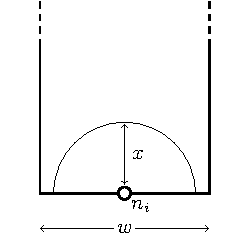
\includegraphics[width=0.4\textwidth]{tikz/geomtr_prb_05.pdf}%
      \hfill
      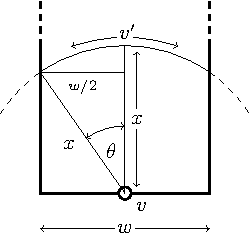
\includegraphics[width=0.4\textwidth]{tikz/geomtr_prb.pdf}% 
    }%
    %\caption{}%??
    \label{fig:geomtr_prb}
  \end{figure}

  For a general $v$ make coordinate transformation

\end{proof}

We can verify this result by computationally extracting the distance
dependencies in the sample graphs generated. 

\begin{figure}[h]
  \centering
  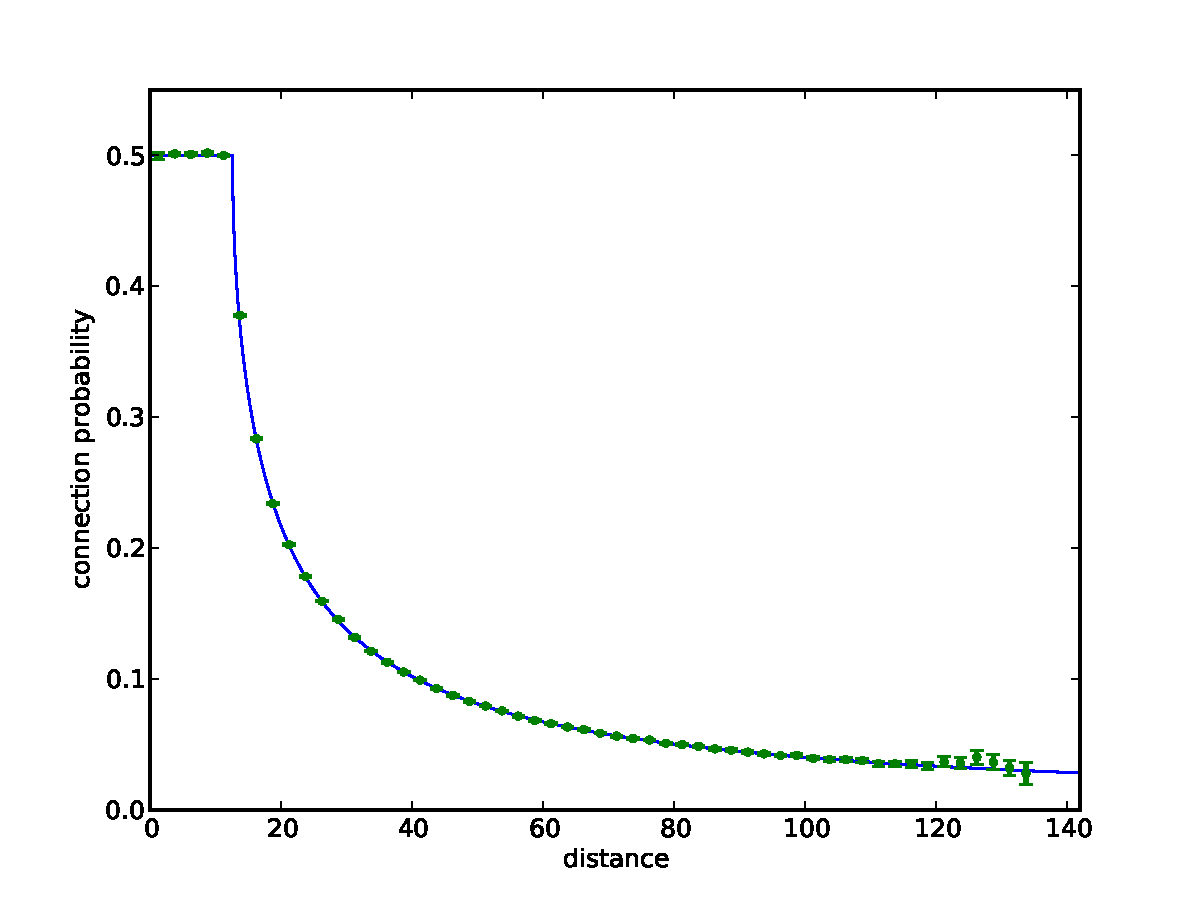
\includegraphics[width=0.7\linewidth]{plots/test.pdf}
  \caption{\textbf{Distance dependent connection probabilities}}%??
  \label{fig:something_else}%??
\end{figure}





\section{Rewiring Methods}

In the network configuration introduced in
section~\ref{sec:network_model} strong directional anisotropy is
present: Edges originating from one node \enquote{point in the same
  direction}, that is they connect to other nodes which cluster around
a. In this section we introduce an algorithm

\vspace{0.5cm}
\begin{figure}[h] 
  \centering 
  \makebox[0.85\textwidth]{%
    %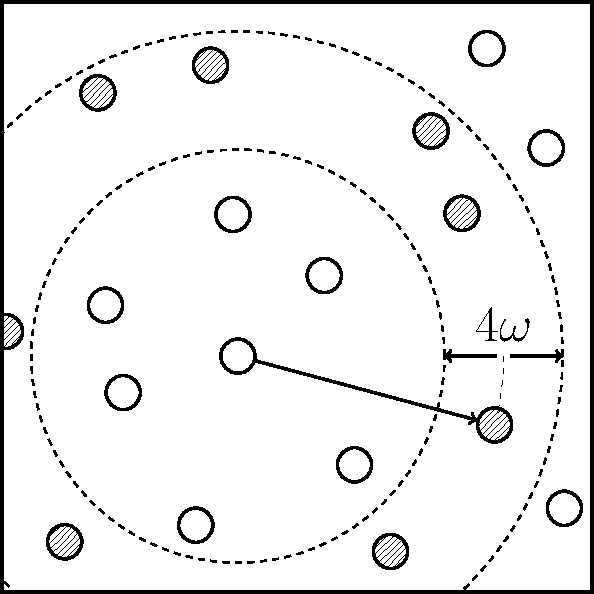
\includegraphics[width=0.4\textwidth]{dist_rew_org.pdf}%
    \begin{overpic}[width=0.4\textwidth]{tikz/distance_rewiring.pdf}
      \put(3,105){\small\textbf{Before}}
    \end{overpic}
    \hfill
    \begin{overpic}[width=0.4\textwidth]{tikz/distance_rewiring.pdf}
      \put(3,105){\small\textbf{After}}
    \end{overpic} 
  }%
  \caption{\textbf{Rewiring}}%??
  \label{fig:distance_rewiring}
\end{figure}

 

\section{Anisotropy Measure}


\section{Summary and Discussion}













%%% Local Variables: 
%%% mode: latex
%%% TeX-master: "../dplths_document"
%%% End: 
